




%%%%%%%%%%%%%%%%%%%%%%%%%%%%%%%%%%%%%%%%%%%%%%%%%%%%%%%%%%%%%%%%%%%%%%%%%
%%%%%%%%%%%%%%%%%%%%%%%%%%%%%%%%%%%%%%%%%%%%%%%%%%%%%%%%%%%%%%%%%%%%%%%%%
%%%%%%%%%%%%%%%%%%%%%%%%%%%%%%%%%%%%%%%%%%%%%%%%%%%%%%%%%%%%%%%%%%%%%%%%%

\begin{frame}{What makes an estimator non-robust?  A tail sum.}

We show that \hspace{1em}
%
%\begin{align*}
$
%
\thetafunlin(\w^*) - \thetafun(\thetahat)  =
{\color{red}
    - \sum_{n=1}^{\lfloor \alpha N \rfloor} \infl_{(n)}
    =:  \noise \shape}
%
$
%\end{align*}
%
\hspace{1em} where \vspace{1em}

\begin{itemize}
\item The ``noise'' $\noise^2 \rightarrow \mathrm{Var}(\sqrt{N}\phi)$
    \begin{itemize}
        \item $\noise^2 = $ is the robust ``sandwich'' variance estimator
        \citep{hampel1986robustbook}
    \end{itemize}
\item The ``shape'' $\shape \le \sqrt{\alpha (1 - \alpha)}$
    determined by $\infl_n$ distribution
    \begin{itemize}
        \item $\shape$ converges to a nonzero constant
    \end{itemize}
\end{itemize}

\begin{center}
\begin{minipage}{0.65\linewidth}
\begin{tikzpicture}
    \onslide<1->{
    \node[anchor=south west,inner sep=0] (image) at (0,0) {
        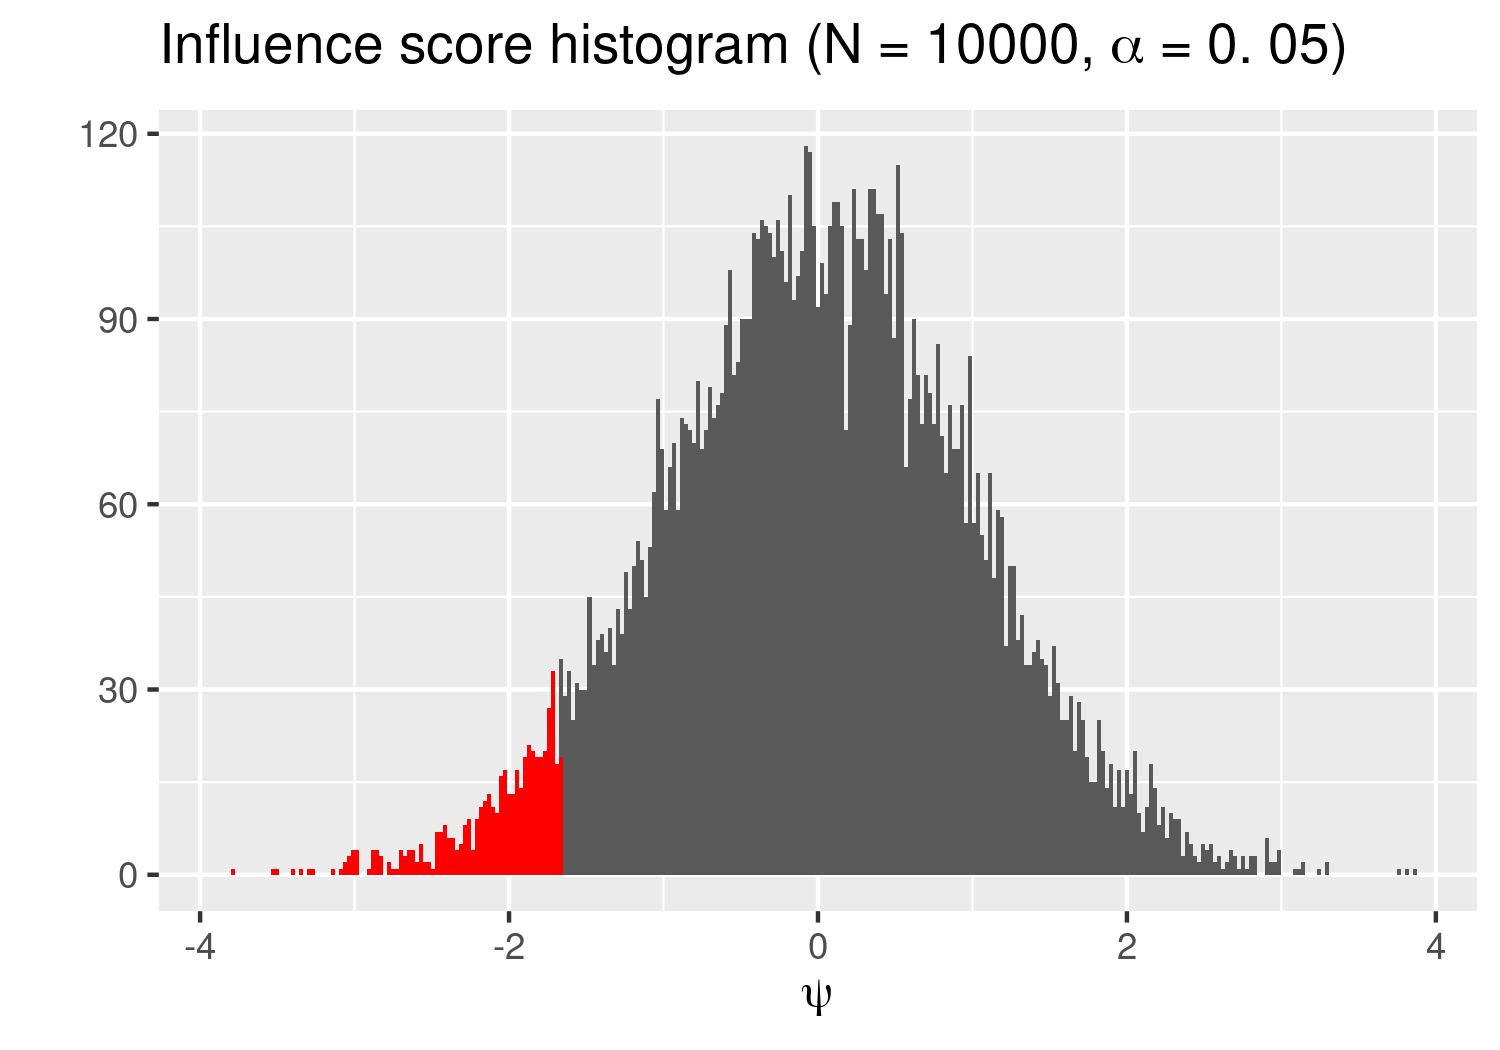
\includegraphics[width=0.98\textwidth]{static_figures/simple_infl_example.png}
    };
    }
    \onslide<1->{
    \begin{scope}[x={(image.south east)},y={(image.north west)}]
        \draw [stealth-stealth][thick][yellow](0.44, 0.4) -- (0.64, 0.4);
    \end{scope}
    \begin{scope}[x={(image.south east)},y={(image.north west)}]
        \draw (0.55,0.38) node[below,yellow][text width=3cm][align=center]
        % {\tiny $\noise$ is controlled by $\var{}{\sqrt{N}\phi(\thetahat)}$};
        {\small $\noise \approx $\\$\var{}{\sqrt{N}\phi(\thetahat)}$};
    \end{scope}
    }
    \onslide<1->{
    \begin{scope}[x={(image.south east)},y={(image.north west)}]
        \draw [stealth-][thick][red](0.3, 0.25) -- (0.3, 0.5);
    \end{scope}
    \begin{scope}[x={(image.south east)},y={(image.north west)}]
        \draw (0.25, 0.5) node[above][text width=3cm][align=center]
        {\small $-\sum_{n=1}^{\lfloor \alpha N \rfloor} \infl_{(n)}$};
    \end{scope}
    }
\end{tikzpicture}
\end{minipage}
\end{center}

\end{frame}



%%%%%%%%%%%%%%%%%%%%%%%%%%%%%%%%%%%%%%%%%%%%%%%%%%%%%%%%%%%%%%%%%%%%%%%%%
%%%%%%%%%%%%%%%%%%%%%%%%%%%%%%%%%%%%%%%%%%%%%%%%%%%%%%%%%%%%%%%%%%%%%%%%%
%%%%%%%%%%%%%%%%%%%%%%%%%%%%%%%%%%%%%%%%%%%%%%%%%%%%%%%%%%%%%%%%%%%%%%%%%

\begin{frame}{Corollaries.}

% {\small
% \textbf{Key quantities:}\\
% \pause $\alpha$  = The proportion of left out points\\
% \pause $\Delta$  = The signal = The change in $\phi$ that would alter your
% conclusion\\
% \pause $\noise^2$ = The noise = A consistent estimator of
% $\mathrm{Var}(\sqrt{N}\phi)$\\
% \pause $\shape$ =
%     The shape = Converges to a nonzero constant, $\le \sqrt{\alpha(1-\alpha)}$\\
% }

Report non-robustness if:
%
\begin{align*}
%
\thetafunlin(\w^*) - \thetafun(\thetahat)  = \noise \shape \ge \Delta
\quad\quad
\Leftrightarrow
\quad\quad
\frac{\Delta}{\noise} \le \shape.
%
\end{align*}
%
We call $\frac{\Delta}{\noise}$ the ``signal to noise ratio.''


\hrulefill

%\vspace{-1em}

\pause
\vspace{0.5em}
\textbf{Corollary:  Non-robustness possible even with correct specification.}
%\vspace{-0.4em}
% {\small The noise $\noise$ may be larger than the effect
% $\Delta$ you're trying to measure.}

\pause
\vspace{0.5em}
\textbf{Corollary:  Leave-$\lfloor \alpha N \rfloor$-out robustness does not vanish as $N \rightarrow \infty$.}
% \vspace{-0.4em}
%
% Both $\shape$ and $\noise$ typically converge to nonzero constants.

\pause
\vspace{0.5em}
Recall that standard errors reject when
$\frac{\Delta}{\noise} \le \frac{1.96}{\sqrt{N}}$.

\pause
\vspace{0.5em}
\textbf{Corollary:  Leave-$\lfloor \alpha N \rfloor$-out is different from standard errors.}
%\vspace{-0.4em}
% $1.96 / \sqrt{N} \ne \shape$

\pause
\vspace{0.5em}
\textbf{Corollary:  Insignificance is always non-robust.}
%\vspace{-0.4em}

Take $\Delta = \frac{1.96 \hat \sigma_\phi}{\sqrt{N}} \rightarrow 0 \le
\shape$.

\pause
\vspace{0.5em}
\textbf{Corollary:  Gross outliers primarily affect robustness
through $\noise$.}
%\vspace{-0.4em}
Cauchy-Schwartz is tight when all the influence scores are the same.

\end{frame}
